\documentclass[proposal]{ugmskripsi}
\usepackage[left=2.5cm, right=2.5cm, top=3cm, bottom=2cm]{geometry}
\usepackage{listings}
\usepackage{xcolor}
\usepackage{float}
\usepackage{graphicx}
\usepackage{amsmath}
\usepackage{comment}
\usepackage[T1]{fontenc}
\usepackage{pgfgantt}

\definecolor{codegreen}{rgb}{0,0.6,0}
\definecolor{codegray}{rgb}{0.5,0.5,0.5}
\definecolor{codepurple}{rgb}{0.58,0,0.82}
\definecolor{backcolour}{rgb}{0.95,0.95,0.92}

\lstset{
  numbers = left, stepnumber=2,
  keywordstyle=\color{blue}\bfseries ,
  numberstyle=\tiny\color{codegray},
  stringstyle=\color{codepurple},
  basicstyle=\ttfamily\footnotesize,
  linewidth = 0.8\textwidth,
  frame=single,
  commentstyle=\color{codegreen}
}

\usepackage[section]{placeins}
\usepackage[colorlinks=true,linkcolor=blue,
            urlcolor=blue,
            citecolor=blue,
            anchorcolor=blue]{hyperref}

\usepackage{makeidx}
\makeindex
\bibpunct{(}{)}{;}{a}{,}{,}

%-----------------------------------------------------------------
% Data Proposal
%-----------------------------------------------------------------
\titleind{Aplikasi Visualisasi Data \textit{Gas While Drilling} untuk Prediksi Tipe Hidrokarbon Menggunakan Algoritma Deterministik}

\titleeng{Gas While Drilling Data Visualization Application for Hydrocarbon Type Prediction Using Deterministic Algorithms}

\fullname{Mohammad Azka Khairur Rahman}

\idnum{23/511608/PA/21830}

\examdate{05 June 2026}

\yearsubmit{2026}

\program{Ilmu Komputer}

\headprogram{Azhari SN}

\dept{Ilmu Komputer dan Elektronika}

\firstsupervisor{Dr. Techn. Khabib Mustofa, S.Si., M.Kom.}

%\secondsupervisor{}

\firstexaminer{}
\secondexaminer{}
\thirdexaminer{}
%-----------------------------------------------------------------

\begin{document}

%-----------------------------------------------------------------
% Bagian Depan
%-----------------------------------------------------------------
\input{bagiandepan.tex}

%-----------------------------------------------------------------
% Abstract
%-----------------------------------------------------------------
%-----------------------------------------------------------------
% Abstract (English)
%-----------------------------------------------------------------
\begin{abstracteng}
Traditional manual hydrocarbon prediction using Gas While Drilling data has long been hindered by inefficiencies and inaccuracies, largely due to human error and the complexity of multi-parameter data analysis. Petrophysical interpretation requires the integration of many variables such as porosity, permeability, resistivity, and saturation, which often makes manual evaluation inconsistent. This study seeks to overcome these limitations by developing a decision support system specifically designed to analyze and visualize Gas While Drilling data in a more intuitive manner. The proposed framework integrates deterministic algorithms with industry-standard petrophysical formulas to process raw well data. The processed data is then presented through intuitive graphical visualizations, enabling geoscientists to identify trends and anomalies more effectively. Furthermore, the system employs rule-based logic to compare derived parameters against established geological thresholds, allowing for a preliminary yet structured prediction of hydrocarbon presence. The system will be capable of distinguishing between hydrocarbon types (e.g., oil or gas) at varying depths, thereby providing more insights into subsurface conditions. This approach not only reduces the risk of human error but also enhances decision-making in exploration and reservoir characterization.

\bigskip
\noindent\textbf{Keywords:} \textit{Hydrocarbon Prediction, Data Visualization, Deterministic Algorithms, Decision Support System.}
\end{abstracteng}


\printindex
\pagenumbering{arabic}

%-----------------------------------------------------------------
% Bab-bab
%-----------------------------------------------------------------
\chapter{INTRODUCTION}

\section{Background}

In the oil and gas industry, subsurface exploration carries immense capital risk \citep{ref3, ref9}. Drilling a single exploration or development well costs millions of dollars; thus, asset teams rely on continuous diagnostic tools to evaluate subsurface formations as drilling advances \citep{ref3}. Globally, rotary drilling is a high-frequency, continuous operation, with thousands of active wells being drilled around the clock across international basins \citep{ref9, ref14, bakerhughes2024}. Because drilling occurs continuously on such a massive operational scale, Gas While Drilling (GWD) analysis has become one of the most essential and widely deployed formation evaluation techniques \citep{ref9, ref12}. GWD measures light-to-heavy hydrocarbon gas fractions ($C_1$ through $C_5$) released into the drilling mud stream as the drill bit cuts through rock layers, providing wellsite geologists with immediate indicators of reservoir fluid content \citep{ref12, haworth1985}. Accurate GWD interpretation enables engineers to confirm hydrocarbon-bearing pay zones quickly or make the critical decision to halt drilling early, thereby saving millions of dollars by avoiding non-productive "dry holes" \citep{ref3, ref9}.

Despite the critical necessity of GWD evaluation during active operations, standard field interpretation workflows remain overly constrained \citep{ref9, ref11}. In prevailing operational practices, wellsite engineers and petrophysicists typically rely on only two basic parameters—the classical Haworth Wetness Ratio ($W_h$) and Balance Ratio ($B_h$)—to evaluate gas shows and classify fluid boundaries \citep{ref12, haworth1985}. Relying solely on this narrow two-ratio pair frequently produces ambiguous or incomplete fluid characterizations, particularly in complex reservoirs with mixed fluid contacts, fluctuating penetration rates, or heavier hydrocarbon components ($C_4$ and $C_5$) that are ignored in simple two-variable evaluations \citep{ref8, ref12, haworth1985}. By restricting evaluation to just $W_h$ and $B_h$, operators miss out on the valuable diagnostic depth offered by modern multi-ratio models, including Pixler ratios, Character ratios, and composite gas-oil indicators \citep{ref13, whittaker1991, spe2020}.

To expand beyond this restricted evaluation and automate multi-parameter log analysis, exploration teams typically look to modern digital platforms \citep{ref1, ref8}. While data-driven machine learning (ML) architectures have been explored for petrophysical prediction \citep{ref4, ref5, ref6}, they act as opaque "black boxes" that fail to expose their internal reasoning \citep{ref1}. Strict industry guidelines, such as \citet{ref3} reserve estimation standards, require step-by-step physical documentation to certify petroleum reserves, meaning non-transparent AI models fail regulatory safety audits and cannot be accepted for official reporting \citep{ref1, ref3}. Conversely, commercial enterprise software suites—such as SLB Techlog or AspenTech Geolog—offer comprehensive, physically grounded formation evaluation tools \citep{ref8, wood2020}. However, these enterprise suites are burdened by cost-prohibitive licensing fees (frequently exceeding tens of thousands of dollars per annual seat license) \citep{ref8, wood2020}. For smaller independent operators, field consultants, wellsite service companies, and academic institutions that specifically require multi-ratio GWD visualization and hydrocarbon fluid typing, purchasing an entire multi-thousand-dollar enterprise suite just to access that specific functionality is financially unfeasible \citep{ref8, ref11, wood2020}.

This situation creates an operational gap: because drilling is conducted frequently and continuously, asset teams urgently need a lightweight, cost-effective tool built specifically for comprehensive GWD visualization and deterministic hydrocarbon classification \citep{ref8, ref11, ref12}. To address this need, this study proposes an open-source, web-based decision support system developed using Python (Dash and Plotly) \citep{ref8}. By integrating classic Haworth wetness and balance ratios with expanded modern formulas into an automated deterministic pipeline, the system rapidly ingests raw mud logs, computes 16 derived gas ratios, classifies fluid zones, and renders interactive vertical area charts in seconds—providing multi-ratio cross-comparison without the financial burden of enterprise software licenses \citep{ref3, ref8, ref11, ref12}.

\subsection{Problem Statement}

Because drilling operations are conducted continuously on a massive global scale, Gas While Drilling (GWD) log evaluation is an essential diagnostic requirement; however, current field practices predominantly depend on a limited two-ratio framework (Haworth Wetness and Balance ratios) that yields ambiguous fluid predictions, while modern alternatives force engineers to choose between non-auditable "black-box" machine learning models or purchasing cost-prohibitive enterprise software suites (such as SLB Techlog or Aspen Geolog) simply to access multi-ratio GWD plotting and evaluation features. Consequently, there is an urgent need for a dedicated, open-source decision support platform that automates multi-ratio GWD data visualization and deterministic hydrocarbon classification in seconds, delivering full mathematical transparency and multi-parameter comparative insights without the burden of expensive corporate software licenses.

\section{Research Objectives}

To design, develop, and deploy an open-source, web-based deterministic decision support application specifically tailored for Gas While Drilling (GWD) log visualization and automated hydrocarbon fluid classification, eliminating the necessity for costly commercial software licenses, non-transparent machine learning models, or oversimplified two-ratio evaluation practices.

To systematically resolve the challenges outlined in the problem statement, the specific research objectives are formulated as follows:

To overcome the diagnostic limitations of relying solely on an oversimplified two-ratio baseline, the first objective is to program a fully auditable deterministic calculation engine in Python. This engine directly ingests raw chromatographic gas fractions ($C_1$ through $C_5$) and automates the calculation of 16 derived petrophysical indicators, expanding beyond standard Wetness and Balance ratios to incorporate classic Pixler ratios, expanded Haworth Character ratios, and composite fluid indicators.

To address the barrier of expensive enterprise software suites and provide comprehensive curve analysis, the second objective is to develop a dedicated, high-fidelity interactive dashboard using Dash and Plotly. That allow users to visually cross-compare legacy two-ratio curves with modern expanded ratio curves side-by-side without needing multi-thousand-dollar commercial licenses.

To satisfy the operational urgency of active, drilling environments, the third objective is to optimize the software pipeline for high computational throughput. The system is engineered to execute the entire end-to-end processing pipeline—spanning file ingestion, data normalization, 16-parameter ratio computation, and multi-track visual rendering—in under 5 seconds across continuous well trajectories spanning thousands of meters of depth.

\section{Research Benefits}

The development of a dedicated, open-source GWD petrophysical application provides direct contributions to active field operations, independent energy entities, and academic environments.

\subsection{Industrial and Operational Impact}

\subsubsection{Cost Reduction and Targeted Feature Access}
By providing a free, web-accessible tool dedicated specifically to comprehensive GWD processing and multi-ratio visual display, this software eliminates the requirement for smaller operators and field consultants to purchase multi-thousand-dollar enterprise licenses (such as SLB Techlog or Aspen Geolog) merely to execute routine GWD interpretations.

\subsubsection{Capital Risk Mitigation and Multi-Ratio Accuracy}
Expanding standard formation evaluation from an oversimplified two-ratio baseline to an integrated 16-parameter deterministic framework provides wellsite teams with significantly sharper fluid differentiation. Hard-coding proven physical equations directly into the software core ensures that every meter drilled is evaluated against consistent mathematical criteria, helping companies protect capital by avoiding non-productive "dry holes".

\subsection{Academic and Educational Contributions}

\subsubsection{Democratization of Petrophysical Tools}
Due to extreme licensing costs associated with enterprise software platforms, university departments and independent researchers are frequently locked out of modern digital log evaluation tools. Deploying an open-source platform democratizes access to multi-ratio petrophysical evaluation tools for classrooms and students.

\subsubsection{Enhancement of Geoscience Education}
In academic settings, students often struggle to connect theoretical gas ratio formulas with actual visual log curves. This application provides a modern, interactive visual platform where students can observe log curve shifts across multiple vintage and modern ratio methods simultaneously as underlying gas parameters change.
\chapter{LITERATURE REVIEW}

\section{Computational Approaches in Hydrocarbon Prediction}

The interpretation of well log and mud log data has historically depended on the expertise and judgment of individual petrophysicists. As reservoirs grow more complex and the volume of acquired data continues to expand, the limitations of purely manual interpretation have become increasingly apparent. Human analysis is inherently time-consuming, difficult to scale, and subject to variability between interpreters. Computational approaches address these limitations directly: they offer systematic, reproducible pipelines capable of processing large multi-well datasets with consistent logic and quantifiable uncertainty. Two broad paradigms have emerged as dominant methodological frameworks in this space --- deterministic algorithmic approaches rooted in established physical laws, and data-driven approaches based on machine learning and deep learning architectures. Both have been demonstrated in the literature to provide meaningful uplift over manual interpretation alone, and an understanding of their respective strengths and constraints is essential for contextualizing the methodology of this study.

\subsection{Deterministic and Algorithmic Approaches}

Deterministic approaches to formation evaluation derive their outputs through the direct application of explicit mathematical models to measured log data. The intellectual foundation of this paradigm can be traced to the seminal work of \citet{archie1942}, who established the empirical relationship between a formation's measured electrical resistivity, its porosity, and the saturation of its pore fluids. This equation, now universally known as Archie's Law, provided the first rigorous quantitative framework for inferring subsurface fluid content from borehole measurements, and it remains a cornerstone of formation evaluation to this day. Subsequent decades brought additional deterministic models addressing shaly sand corrections (the Simandoux equation), volumetric mineral decomposition, and the interpretation of nuclear and acoustic logs --- all of which operate on the same fundamental principle: given a set of calibrated input measurements and known physical relationships, the output can be computed directly and reproduced exactly \citep{ref9, ref11}.

A defining characteristic of deterministic methods is their full transparency. Every intermediate result can be audited, the sensitivity of the output to each input parameter can be quantified, and any experienced petrophysicist can trace the chain of reasoning from raw log reading to final reservoir classification. This auditability is not merely an academic advantage; it is often a regulatory and commercial requirement. The \citet{ref3} standards for petroleum resource estimation, for instance, explicitly distinguish deterministic from probabilistic assessment procedures and require that the methodology underlying any reserves declaration be clearly documented and defensible. A code-based deterministic system --- one in which Archie's Law, shale volume corrections, and pay-zone criteria are encoded as explicit algorithmic rules --- inherently satisfies this requirement \citep{ref11}.

The practical implementation of deterministic petrophysical logic in software has a long history. Early systems encoded expert knowledge as lookup tables and threshold-based decision trees. More sophisticated modern implementations use layered conditional logic that integrates multiple log curves simultaneously --- for instance, cross-referencing gamma ray for lithology discrimination, resistivity for fluid identification, and neutron-density crossplots for porosity calibration --- to classify each depth interval. The transparency of such rule-based systems means that domain experts can inspect, challenge, and refine the underlying logic iteratively, which is particularly valuable in frontier basins where geological priors are poorly constrained. The primary limitation of purely deterministic approaches is their rigidity: the accuracy of the output is bounded by the validity of the underlying physical model, and classical equations like Archie's Law carry known assumptions (clean formations, water-wet pores, homogeneous lithology) that are frequently violated in complex reservoirs \citep{ref9, ref11}.

\subsection{Machine Learning and Data-Driven Approaches}

Parallel to deterministic methods, the application of machine learning (ML) and deep learning (DL) to formation evaluation and hydrocarbon prediction has grown substantially since its early introduction to petroleum engineering. The conceptual groundwork for applying artificial intelligence techniques to oilfield problems was laid by \citet{ref1}, who demonstrated that artificial neural networks could approximate complex, non-linear mappings between well log inputs and reservoir properties that resist explicit physical formulation. That early work catalysed a sustained research trajectory that has since expanded to include Random Forests, Support Vector Machines, gradient-boosted tree ensembles, and convolutional and recurrent neural network architectures.

The primary appeal of ML approaches is their ability to learn structure directly from data without requiring the analyst to specify the functional form of the relationship between input and output. In heterogeneous reservoirs where the porosity--permeability relationship is non-stationary, where lithological facies change rapidly along the wellbore, or where the applicability of classical deterministic equations is uncertain, ML models can often achieve higher predictive accuracy than their physics-based counterparts. This has been demonstrated across a range of formation evaluation tasks. \citet{ref5} showed that ML models trained on wireline log suites can predict in-situ geomechanical properties with strong accuracy, highlighting the utility of data-driven methods in applications where direct measurement is prohibitively expensive. The task of reconstructing missing or degraded log intervals --- a common practical problem in older wells or in wells where certain tools were not run --- has similarly been addressed through DL architectures. \citet{ref6} introduced a flexible graph-neural-network approach, FlexLogNet, capable of predicting any arbitrary missing log from the remaining available logs within the same well, adaptively adjusting its input configuration to whatever data is present. Well-log completion methods of this type have become increasingly important as operators attempt to extract maximum value from legacy datasets containing incomplete log suites \citep{ref4, ref6}.

Despite these demonstrated capabilities, ML and DL approaches carry inherent limitations that are particularly consequential in a high-stakes petroleum context. The most widely cited of these is the interpretability problem: because complex neural networks and ensemble models derive their predictions through high-dimensional, non-linear transformations that are not straightforwardly human-readable, it can be difficult or impossible to explain why a specific prediction was generated. This opacity creates friction in professional and regulatory settings, where the basis for any reservoir characterization must be auditable \citep{ref8}. A second major constraint is data dependency: supervised ML models require sufficient labelled training examples to generalise reliably to unseen wells. In frontier exploration areas, where few wells have been drilled and production data is scarce, the training data volumes required to fit complex models may simply not be available, limiting their practical applicability \citep{ref1}. A third concern is distribution shift: models trained on data from one geological province may perform poorly when applied to a different basin with distinct lithological characteristics, even if the surface log signatures appear superficially similar.
\chapter{RESEARCH METHODOLOGY}

\section{Research Design and Software Engineering Life Cycle}

This research develops an open-source, web-based decision support system designed to automate the ingestion, multi-ratio petrophysical analysis, real-time visualization, and deterministic fluid forecasting of Gas While Drilling (GWD) data. Because the platform delivers an interactive computational tool for operational geoscience, the methodology follows a structured five-stage Software Development Life Cycle (SDLC) adapted for scientific computing:

\begin{enumerate}
    \item \textbf{Requirements Analysis and Specification:} Formulating functional requirements (multi-format mud log parsing, automated 16-parameter ratio computation, deterministic fluid classification, and 21-track depth-registered visualization) and non-functional requirements (sub-5-second processing latency, mathematical auditability, and open-source accessibility). Requirements were established through domain feedback from practicing petrophysicists, operations geologists, and wellsite engineers.
    
    \item \textbf{System and Architectural Design:} Structuring the platform using a decoupled three-tier software architecture comprising a Data Ingestion Layer, a Deterministic Logic Engine Layer, and a Reactive Presentation Layer. The core calculation pipeline models petrophysical dependencies as a declarative directed acyclic graph, supporting dynamic parameter customization and live schema management.
    
    \item \textbf{Software Implementation:} Implementing modular Python packages (\texttt{parser.py}, \texttt{engine.py}, \texttt{evaluator.py}, and \texttt{app.py}) using vectorized numerical routines (NumPy, Pandas) and reactive web components (Dash, Plotly). Because the calculation core operates strictly on closed-form petrophysical formulas and explicit boundary thresholds, the system undergoes a data-free deterministic build phase requiring no stochastic model training.
    
    \item \textbf{System Verification and Multi-Tier Evaluation:} Conducting comprehensive validation spanning algorithmic unit verification against analytical reference values, empirical classification benchmarking against ground-truth well tests using multi-class classification metrics (Accuracy, Precision, Recall, Macro-$F_1$) \citep{sokolova2009, powers2011}, computational latency profiling ($\Delta t_{\text{total}} \le 5.0\text{ s}$), and observational user testing ($S_{\text{user}} > 68.0$).
    
    \item \textbf{Packaging and Open-Source Deployment:} Assembling standardized environment manifests (\texttt{requirements.txt}) and releasing the source code on a public repository to facilitate reproducible formation evaluation and academic research.
\end{enumerate}

\section{Requirements Analysis and Specification}

Establishing structured software specifications ensures that the developed application addresses operational challenges in formation evaluation while maintaining computational efficiency and system reliability.

\subsection{Functional Requirements (FR)}
The functional specifications define the operational capabilities delivered by the system:
\begin{itemize}
    \item \textbf{FR-01 (Multi-Format Ingestion):} Ingest raw mud logging files across standard tabular and delimited text formats (\texttt{.txt}, \texttt{.csv}, \texttt{.xlsx}, and \texttt{.las}), automatically isolating data records from variable company headers.
    \item \textbf{FR-02 (Continuous Data Normalization):} Validate, align, and clean chromatographic gas curves ($C_1$ through $C_5$) against continuous Measured Depth ($MD$) indices, systematically handling missing or non-positive values.
    \item \textbf{FR-03 (Automated Multi-Ratio Computation):} Automatically compute 16 derived petrophysical indicators from input gas curves upon file upload.
    \item \textbf{FR-04 (Deterministic Fluid Zone Forecasting):} Apply closed-form decision-tree logic to classify depth increments into categorical fluid regimes: Gas Zone, Oil Zone, or Water/Non-Productive Sand.
    \item \textbf{FR-05 (Multi-Track Depth-Synchronized Visualization):} Render continuous vertical area charts for all computed indicators and fluid zones across 21 dedicated tracks, featuring synchronized scrolling, depth zooming, and cursor tooltips.
    \item \textbf{FR-06 (Dynamic Schema and Formula Management):} Enable interactive column visibility toggling, track reordering, and live formula and cutoff threshold customization with immediate preview updates.
    \item \textbf{FR-07 (Data Export and Reporting):} Enable the export of computed petrophysical curves and classification summaries in standardized tabular formats.
\end{itemize}

\subsection{Non-Functional Requirements (NFR)}
Non-functional specifications ensure software robustness, responsiveness, and professional auditability:
\begin{itemize}
    \item \textbf{NFR-01 (Computational Latency):} The end-to-end execution pipeline (file ingestion, ratio calculation, and multi-track visual rendering) must complete in under 5.0 seconds for well trajectories exceeding 3,000 meters.
    \item \textbf{NFR-02 (Mathematical Auditability):} All calculations must operate on explicit, transparent formulas with zero non-traceable parameters, ensuring complete compliance with SPE PRMS reserve certification standards \citep{ref3}.
    \item \textbf{NFR-03 (Usability and Workflow Learnability):} The interface must deliver an intuitive single-click operational workflow accessible without specialized software training, targeting a mean usability score of $\overline{S} > 68.0/100$.
    \item \textbf{NFR-04 (Accessibility and Open Distribution):} The application must run on open-source Python technologies, eliminating multi-thousand-dollar annual commercial licensing constraints \citep{wood2020}.
\end{itemize}

\subsection{Requirements Elicitation}
Requirements were synthesized through domain surveys and consultations with practicing wellsite engineers, operations geologists, and petrophysicists. The feedback highlighted operational preferences for instantaneous multi-ratio cross-comparison, customizable threshold cutoffs, and responsive multi-track visual layouts that mirror standardized wellsite strip log templates.

\section{System Architecture and Design}

To ensure separation of concerns, high maintainability, and low computational overhead, the software is structured as a decoupled three-tier architecture.

\subsection{Three-Tier Architectural Overview}
The system architecture separates data processing into three dedicated layers:
\begin{enumerate}
    \item \textbf{Data Parsing \& Ingestion Layer (\texttt{parser.py}):} Handles file decoding, format identification, header stripping, data cleaning, and structured matrix generation.
    \item \textbf{Deterministic Logic Engine Layer (\texttt{engine.py} \& \texttt{evaluator.py}):} Implements petrophysical formulas, maintains the declarative parameter dependency graph, vectorizes numerical operations, and executes zone classification logic.
    \item \textbf{Presentation \& Dashboard Layer (\texttt{app.py}):} Provides an interactive, reactive web user interface built with Dash and Plotly, delivering responsive layout controls and synchronized multi-track visual rendering.
\end{enumerate}

\subsection{Data Parsing \& Ingestion Layer Design}

The ingestion module isolates valid numeric data matrices from raw well logs through a two-stage pipeline:

\begin{enumerate}
    \item \textbf{Metadata and Header Isolation:} Mud log files frequently contain unstructured operator comments and variable metadata headers. The parser scans the incoming data stream line-by-line using keyword triggers (such as \texttt{\char`~A} in LAS files or standard column tokens like \texttt{Depth} and \texttt{MD}) to isolate the numerical tabular matrix.
    \item \textbf{Data Normalization and Type Casting:} Delimited data lines are parsed, stripped of non-numeric formatting characters, and converted into continuous float matrices indexed by measured depth ($MD$). Missing or anomalous data points are systematically handled to preserve calculation continuity.
\end{enumerate}

\subsection{Declarative Parameter Dependency Graph and Indicator Pipeline}

To ensure flexibility across diverse geological basins without requiring code-level modifications, the computation engine represents petrophysical variables, mathematical formulas, and decision boundaries as a \textbf{declarative directed acyclic graph (DAG)}. In this structural representation:
\begin{itemize}
    \item \textbf{Vertices} represent physical data channels, encompassing measured gas curves ($C_1$, $C_2$, $C_3$, $iC_4$, $nC_4$, $iC_5$, $nC_5$), derived ratio parameters ($W_h$, $B_h$, $C_h$, $R_1 \dots R_5$, $DR$, $I_{\text{carbon}}$), composite indicators ($GOW, WBS, GOR$), and categorical fluid classification states.
    \item \textbf{Edges} define mathematical dependencies, functional transformations, and boundary decision logic connecting parent curves to downstream petrophysical indicators.
\end{itemize}

This decoupled, declarative structure allows the computation engine to dynamically re-evaluate calculation paths in memory when formula expressions or classification cutoffs are adjusted through the interface, ensuring mathematical transparency and regional adaptivity.

\subsubsection{The 16 Derived Petrophysical Indicators}
The data pipeline processes measured chromatographic gas curves to evaluate 16 derived parameters:

\paragraph{1--5. Classic and Expanded Pixler Ratios \citep{ref13}:}
Evaluates light-to-medium hydrocarbon fractions to delineate gas from oil regimes:
\begin{equation}
    R_1 = \frac{C_1}{C_2}, \quad R_2 = \frac{C_1}{C_3}, \quad R_3 = \frac{C_2}{C_3}, \quad R_4 = \frac{C_1}{C_4}, \quad R_5 = \frac{C_1}{C_5}
\end{equation}

\paragraph{6--7. Expanded Butane Isomer Multipliers:}
Tracks methane against separated butane isomers to capture sensitivity to heavier, liquid-associated hydrocarbon fractions:
\begin{equation}
    \text{Ratio}_{\text{iC4}} = \frac{C_1}{iC_4}, \quad \text{Ratio}_{\text{nC4}} = \frac{C_1}{nC_4}
\end{equation}

\paragraph{10. Total Gas Volume ($TG$) \citep{ref14}:}
Calculated by summing all recorded hydrocarbon gas fractions when Total Gas is not pre-recorded in the field log:
\begin{equation}
    TG = C_1 + C_2 + C_3 + iC_4 + nC_4 + iC_5 + nC_5
\end{equation}

\paragraph{11. Dryness Ratio ($DR$):}
Quantifies the methane fraction within the total hydrocarbon gas mixture:
\begin{equation}
    DR = \frac{C_1}{TG}
\end{equation}

\paragraph{12. Carbon-Weighted Density Index ($I_{\text{carbon}}$):}
Quantifies carbon density across the gas stream, scaled by carbon atom count:
\begin{equation}
    I_{\text{carbon}} = \frac{TG}{C_1 + 2C_2 + 3C_3 + 4iC_4 + 4nC_4 + 5iC_5 + 5nC_5}
\end{equation}

\paragraph{13--15. Expanded Haworth Show Evaluation Ratios \citep{haworth1985, ref12}:}
These three expanded parameters form the core fluid-typing decision framework (Wetness $W_h$, Balance $B_h$, and Character $C_h$):
\begin{equation}
    W_h = \left( \frac{C_2 + C_3 + iC_4 + nC_4 + iC_5 + nC_5}{TG} \right) \times 100
\end{equation}
\begin{equation}
    B_h = \frac{C_1 + C_2}{C_3 + iC_4 + nC_4 + iC_5 + nC_5}
\end{equation}
\begin{equation}
    C_h = \frac{iC_4 + nC_4 + iC_5 + nC_5}{C_3}
\end{equation}

\paragraph{16. Composite Screening Indicators ($GOW, WBS, GOR$) \citep{whittaker1991, spe2020}:}
Continuous composite indicators isolate heavy fluid concentrations and decouple total gas fluctuations:
\begin{equation}
\begin{aligned}
    \text{GOW} &= \frac{(\text{C}_3 + \text{iC}_4 + \text{iC}_5 + \text{nC}_4 + \text{nC}_5) \cdot \text{TG}}{\text{C}_1 + \text{C}_2 + \text{C}_3 + \text{iC}_4 + \text{iC}_5 + \text{nC}_4 + \text{nC}_5}, \\[1ex]
    \text{GOW}_{\text{noTG}} &= \frac{\text{C}_3 + \text{iC}_4 + \text{iC}_5 + \text{nC}_4 + \text{nC}_5}{\text{C}_1 + \text{C}_2 + \text{C}_3 + \text{iC}_4 + \text{iC}_5 + \text{nC}_4 + \text{nC}_5}
\end{aligned}
\end{equation}
\begin{equation}
    WBS = \frac{\log(B_h) - 0.903}{2.097} - \frac{\log(W_h)}{2}
\end{equation}
\begin{equation}
    GOR = \begin{cases} 0 & \text{if } 0.8 < TG < 1.2 \text{ and } C_1 > 2000 \text{ ppm} \\ 1 & \text{otherwise} \end{cases}
\end{equation}

These 16 multi-ratio outputs feed into a deterministic rule matrix \citep{ref1} that classifies every depth increment into categorical zones: "Gas Zone," "Oil Zone," or "Water/Non-Productive Zone."

\subsection{User Interface \& Visualization Architecture Design}

The presentation layer is built with the \textit{Dash Python Framework} and \textit{dash-bootstrap-components} (\texttt{dbc}) to deliver a responsive, web-based analytics environment:

\begin{itemize}
    \item \textbf{Reactive Pipeline (\texttt{app.callback}):} Asynchronous callbacks capture user interactions, triggering calculation pipelines in memory and updating visual tracks without full-page reloads.
    \item \textbf{Containerized Controls (\texttt{dcc.Upload} \& \texttt{dbc.Modal}):} Ingestion controls, column configurations, and formula settings are containerized in modal interfaces to maintain a focused visualization workspace.
    \item \textbf{Multi-Track Plotly Visualizations:} Processed indicators and fluid classification overlays are rendered across 21 dedicated vertical subplots synchronized along the Measured Depth ($MD$) axis.
\end{itemize}

\subsection{User Interface Architecture and Workflow Design}

The interface is structured to streamline formation evaluation into a direct, visually intuitive workflow while providing flexible configuration options for operational geoscientists.

\subsubsection{Visual Interface Design}
The visual layout and interactive components of the application are shown in the following interface designs:

\begin{figure}[H]
    \centering
    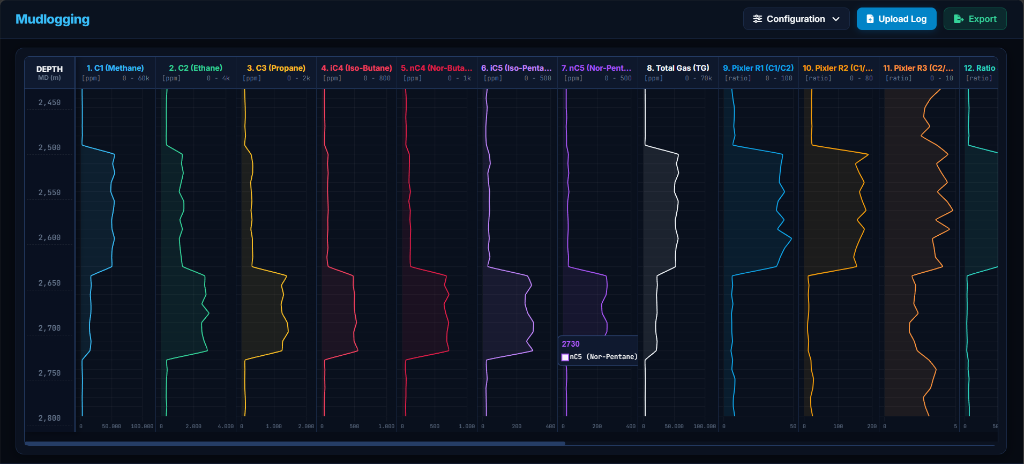
\includegraphics[width=\textwidth]{mockup_main_tracks.png}
    \caption{Main Application Interface featuring the 21-track continuous well log visualization with pinned left-hand Measured Depth ($MD$) axis and synchronous crosshair cursor.}
    \label{fig:mockup_main}
\end{figure}

\begin{figure}[H]
    \centering
    \begin{minipage}[t]{0.48\textwidth}
        \centering
        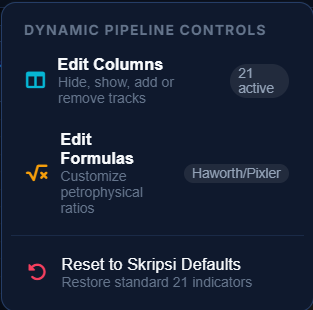
\includegraphics[width=\textwidth]{mockup_config_dropdown.png}
        \caption{Pipeline Controls dropdown menu in the top navigation bar.}
        \label{fig:mockup_config}
    \end{minipage}
    \hfill
    \begin{minipage}[t]{0.48\textwidth}
        \centering
        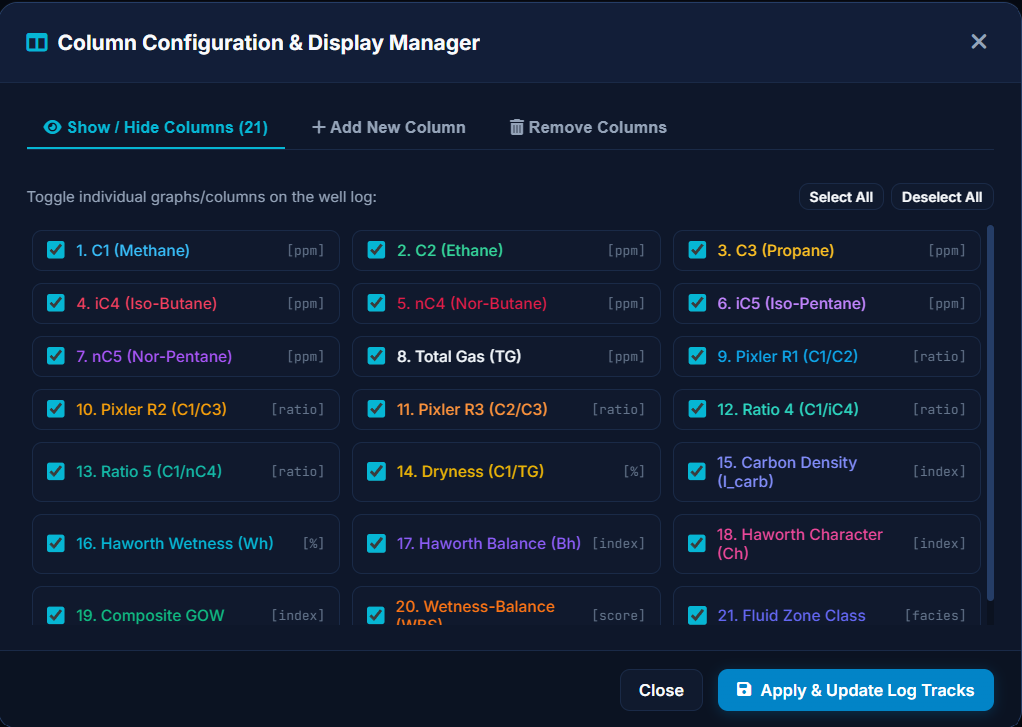
\includegraphics[width=\textwidth]{mockup_columns_manager.png}
        \caption{Column Configuration \& Display Manager modal for toggling and reordering tracks.}
        \label{fig:mockup_columns}
    \end{minipage}
\end{figure}

\begin{figure}[H]
    \centering
    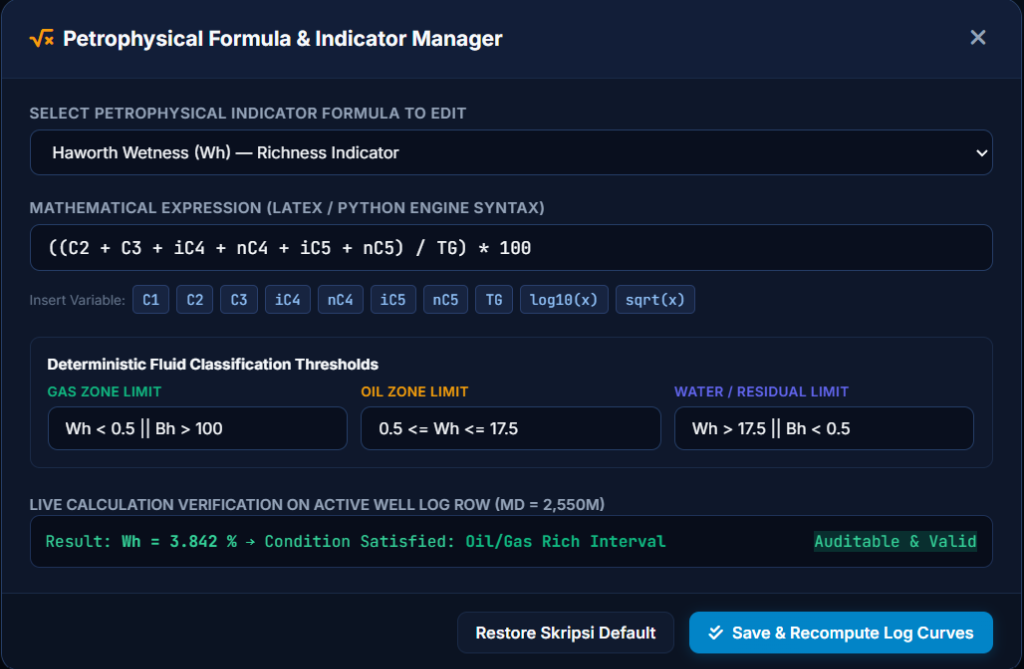
\includegraphics[width=0.88\textwidth]{mockup_formulas_manager.png}
    \caption{Petrophysical Formula \& Indicator Manager modal for live mathematical editing, variable insertion, threshold tuning, and real-time calculation preview.}
    \label{fig:mockup_formulas}
\end{figure}

\subsubsection{End-User Operational Workflow}

The application workflow is structured across four sequential stages designed to minimize operational friction:

\begin{enumerate}
    \item \textbf{Data Ingestion:} 
    The user uploads a mud logging or well logging file (\texttt{.csv}, \texttt{.txt}, \texttt{.xlsx}, or \texttt{.las}) through the file uploader. The ingestion pipeline extracts gas channels ($C_1 - C_5, TG$), normalizes depth measurements, calculates the 16 derived petrophysical indicators, executes fluid classification, and renders the 21-track visualization in under 5 seconds.

    \item \textbf{Well Log Exploration:} 
    Users analyze continuous depth trajectories with synchronized multi-track scrolling locked to the Measured Depth ($MD$) axis, inspecting numerical values via hover crosshairs and reviewing color-coded fluid zone classification overlays.

    \item \textbf{Track Display Customization (Edit Columns):} 
    Accessing the \textit{Column Configuration \& Display Manager} (Figure~\ref{fig:mockup_columns}) enables users to toggle the visibility of individual parameter tracks, adjust column sequences, and manage dataset schemas with immediate live updates.

    \item \textbf{Formula and Threshold Calibration (Edit Formulas):} 
    Through the \textit{Petrophysical Formula \& Indicator Manager} (Figure~\ref{fig:mockup_formulas}), users can modify indicator mathematical expressions using quick-insert variable tokens (e.g., $C_1 \dots C_5, TG, W_h, B_h, \log_{10}$), adjust classification cutoffs, and preview calculations live against active well log records.
\end{enumerate}

\section{Software Implementation}

The implementation translates the architectural design into modular, clean, and maintainable Python packages adhering to scientific software standards.

\subsection{Module Responsibilities}
The codebase is structured into four primary modules:
\begin{itemize}
    \item \texttt{parser.py}: Implements file decoding, format detection, header stripping, and missing-value normalization.
    \item \texttt{engine.py}: Encapsulates the declarative parameter graph, vectorized petrophysical formula pipelines, and deterministic fluid classification routines.
    \item \texttt{evaluator.py}: Houses ground-truth validation routines, confusion matrix calculation, and statistical performance benchmarking.
    \item \texttt{app.py}: Configures Dash application callbacks, binds user interactions, and renders responsive multi-track visual components.
\end{itemize}

\subsection{Deterministic Implementation Principles}
Because the calculation engine is purely deterministic—operating strictly on closed-form petrophysical formulas and explicit boundary thresholds—the system development requires no empirical training data or stochastic model fitting during construction. Algorithms are validated directly against analytical test matrices to guarantee mathematical fidelity.

\subsection{In-Memory Reactive State Execution}
The application executes entirely in memory. Uploaded well data is parsed, processed through vectorized NumPy and Pandas routines, and rendered across synchronized Plotly subplots, ensuring rapid execution without persistent server-side caching.

\section{System Verification and Performance Evaluation}

Validation follows a structured evaluation strategy covering four core dimensions: mathematical correctness, empirical classification accuracy, computational latency, and user experience.

\subsection{Algorithmic Unit Verification}
Algorithmic verification confirms that all coded formulas match their analytical mathematical definitions. Unit tests run against synthetic benchmark tensors with predefined inputs and outputs, ensuring zero floating-point drift or calculation errors across all 16 ratio indicators.

\subsection{Empirical Classification Accuracy and Ground-Truth Validation}
To evaluate the predictive correctness of the deterministic fluid classification engine, model predictions are benchmarked against ground-truth reservoir fluid contacts established by Wireline Formation Testers (RFT/MDT) and production well tests. The multi-class classification problem is evaluated across three primary reservoir fluid regimes:
\begin{equation}
    C = \{\text{Gas Zone}, \text{Oil Zone}, \text{Water / Non-Productive Sand}\}
\end{equation}

For each class $c \in C$, depth intervals are categorized in a confusion matrix as True Positives ($TP_c$), False Positives ($FP_c$), True Negatives ($TN_c$), and False Negatives ($FN_c$). Performance is quantified using standard classification metrics \citep{sokolova2009, powers2011}:

\begin{enumerate}
    \item \textbf{Overall Classification Accuracy:} Measures the total proportion of depth intervals correctly classified across all categories:
    \begin{equation}
        \text{Accuracy} = \frac{\sum_{c \in C} TP_c}{\sum_{c \in C} (TP_c + FP_c + FN_c)}
    \end{equation}

    \item \textbf{Precision (Positive Predictive Value):} Quantifies the proportion of predicted class $c$ intervals that are true reservoir pay zones:
    \begin{equation}
        \text{Precision}_c = \frac{TP_c}{TP_c + FP_c}
    \end{equation}

    \item \textbf{Recall (Sensitivity / True Positive Rate):} Measures the proportion of actual occurrences of fluid class $c$ correctly identified by the system:
    \begin{equation}
        \text{Recall}_c = \frac{TP_c}{TP_c + FN_c}
    \end{equation}

    \item \textbf{Class F1-Score:} The harmonic mean of Precision and Recall for class $c$:
    \begin{equation}
        F_{1, c} = 2 \times \frac{\text{Precision}_c \times \text{Recall}_c}{\text{Precision}_c + \text{Recall}_c}
    \end{equation}

    \item \textbf{Macro-Averaged F1-Score ($\text{Macro-}F_1$):} Provides an unweighted mean of F1-Scores across all classes, ensuring that minority classes (e.g., thin oil-bearing pay intervals) are evaluated with equal importance relative to dominant non-productive intervals \citep{sokolova2009}:
    \begin{equation}
        \text{Macro-}F_1 = \frac{1}{|C|} \sum_{c \in C} F_{1, c}
    \end{equation}
\end{enumerate}

\subsection{Computational Throughput Benchmarking ($\Delta t_{\text{total}} \le 5.0\text{ s}$)}
To evaluate operational speed in active wellsite environments, system efficiency is measured across the complete end-to-end processing pipeline:
\begin{equation}
    \Delta t_{\text{total}} = t_{\text{ingest}} + t_{\text{compute}} + t_{\text{render}}
\end{equation}
The target benchmark requires $\Delta t_{\text{total}} \le 5.0\text{ seconds}$ when processing dense mud logging datasets spanning full well trajectories ($> 3000\text{ m}$).

\subsection{User Experience and Usability Evaluation}

To assess operational usability, navigation fluency, and interface clarity, evaluation combines observational analysis with standardized usability benchmarking:

\subsubsection{Task-Oriented Behavioral Observation}
Domain practitioners (petrophysicists, operations geologists, and wellsite engineers) are observed during structured interpretation sessions using direct observation, interaction telemetry, and concurrent \textit{Think-Aloud Protocols} across four core workflows:
\begin{enumerate}
    \item \textbf{Data Ingestion Workflow:} Uploading raw field mud logs and observing automated channel detection. Evaluators' time-to-first-render and initial navigation choices are tracked.
    \item \textbf{Multi-Track Interpretation Workflow:} Inspecting continuous vertical tracks, utilizing crosshair tooltips, and identifying predicted fluid contacts.
    \item \textbf{Column Management Workflow:} Accessing the *Column Configuration Manager* to isolate targeted ratio groups and customize display layouts.
    \item \textbf{Formula and Threshold Tuning Workflow:} Utilizing the *Petrophysical Formula Manager* to modify indicator equations or adjust classification cutoffs with live preview verification.
\end{enumerate}

\subsubsection{Standardized Usability Benchmarking}
Following the observation session, participants complete a standardized evaluation questionnaire consisting of 10 targeted usability items rated on a linear scale from 1 (poor) to 10 (excellent). An evaluator's total score ($S_{\text{user}}$) is calculated by summing their ratings across all 10 items:
\begin{equation}
    S_{\text{user}} = \sum_{i=1}^{10} q_i
\end{equation}
where $q_i \in [1, 10]$ represents the rating for item $i$. The overall usability performance is measured by the average score ($\overline{S}$) across all $N$ evaluators:
\begin{equation}
    \overline{S} = \frac{1}{N} \sum_{k=1}^{N} S_{\text{user}, k}
\end{equation}
The benchmark target for the system is established at a mean total usability score of $\overline{S} > 68.0$ out of 100.

\section{Software Release and Deployment}

The final SDLC phase encompasses dependency management, software packaging, and open-source distribution.

\subsection{Packaging and Dependency Management}
Software dependencies are specified in a version-pinned \texttt{requirements.txt} manifest covering core libraries (\texttt{dash}, \texttt{dash-bootstrap-components}, \texttt{plotly}, \texttt{pandas}, \texttt{numpy}, and \texttt{openpyxl}), ensuring cross-platform reproducibility across Windows, Linux, and macOS environments.

\subsection{Open-Source Distribution and Accessibility}
The software is published under an open-source license on a public GitHub repository. The repository includes full source code, installation guides, dataset templates, and documentation to support transparent community verification and academic research in formation evaluation.
\chapter{Research Timeline}

This chapter presents the planned schedule for the development and evaluation
of the hydrocarbon zone classification system, spanning five months from July
to November. The work is organized into eight phases that follow the
structure established in the methodology: literature consolidation, data
preparation, algorithmic development, interface construction, testing, and
final documentation.

\section{Phase Descriptions}

\subsection*{Literature Review \& Finalization (July)}
The opening phase consolidates the theoretical grounding of the research.
This includes a final review of the Pixler ratio framework \cite{ref13},
the Haworth--Whittaker composite indicators \cite{haworth1984, haworth1985},
and existing mud logging interpretation workflows. Any gaps identified in
the literature, particularly regarding the GOW, WBS, and GOR indicators are addressed before development begins. Deliverable: annotated bibliography and finalized Chapter 2.

\subsection*{Schema Definition (July--August)}
The structural architecture of the data is formally established by defining the expected column schema. This schema explicitly specifies the depth index alongside the seven required alkane components: Methane ($C_1$), Ethane ($C_2$), Propane ($C_3$), Iso-Butane ($iC_4$), Normal-Butane ($nC_4$), Iso-Pentane ($iC_5$), and Normal-Pentane ($nC_5$). Deliverable: Defined Schema Architecture

\subsection*{System Architecture Design (July--August)}
Before implementation begins, the three-layer architecture (parsing layer,
logic layer, UI layer) is designed in detail. This includes specifying the
data flow between layers, the callback structure for the Dash application,
and the classification threshold table for the majority-vote engine.
Deliverable: architecture document and pseudocode for the classification
pipeline.

\subsection*{Data Parsing \& Standardization Module (August)}
The first implementation phase covers the ingestion pipeline described in
Section~3.1: file upload handling, column validation, null filtering, and
z-score normalization.
Deliverable: working parsing module.

\subsection*{Algorithm \& Classification Logic (August--September)}
All fourteen hydrocarbon indicators (Pixler ratios, Haworth--Whittaker
ratios, TG, GOW, GOW No TG, WBS, GOR) are implemented and verified against
hand-computed reference values. The majority-vote classification engine is
then built on top of the indicator outputs, along with the tie-breaking
priority rule.
Deliverable: fully tested indicator and classification modules.

\subsection*{UI \& Visualization Development (September)}
The Dash application shell, upload modal, and results dashboard are built.
Area charts of each indicator trace and the colour-coded zone overlay are
implemented in Plotly. The interface is validated against the parsed dataset
from Phase 4.
Deliverable: integrated Dash application with end-to-end data flow.

\subsection*{System Testing \& Evaluation (October)}
The complete system is evaluated against the ground-truth well-test labels
using the classification metrics defined in Chapter~3: macro-averaged
Accuracy, Precision, Recall, and F1-Score. The confusion matrix per zone
class is computed, and performance on minority classes (e.g.\ oil-bearing
intervals) is examined in detail. Any misclassification patterns identified
are traced back to individual indicators for potential threshold adjustment.
Deliverable: evaluation results and performance tables for Chapter 4.

\subsection*{Writing, Revision \& Submission (October--November)}
Concurrent with testing in October, revisions are done in response
to supervisor feedback. Chapter 4 (Results) and Chapter 5 (Discussion and
Conclusion) are drafted once evaluation results are available. A full
manuscript review is conducted in early November, followed by final
proofreading and submission by the end of November.
Deliverable: submitted thesis manuscript.

% ------------------------------------------------------------------
\section{Gantt Chart}

Table~\ref{tab:gantt} presents the Gantt chart summarizing the timeline
described above. The horizontal axis spans twenty weeks divided into five
monthly blocks (July through November). Each bar represents the planned
active duration of its corresponding phase; overlapping bars indicate
concurrent work.

\bigskip

\begin{figure}[H]
\centering
\begin{ganttchart}[
    hgrid,
    vgrid,
    x unit=2.2cm,
    y unit title=0.65cm,
    y unit chart=0.7cm,
    title height=1,
    bar height=0.5,
    bar/.append style={fill=blue!25, rounded corners=2pt},
    title label font=\small\bfseries,
    bar label font=\small,
    bar label node/.append style={text width=5.2cm, align=left},
]{1}{5}
  \gantttitle{July}{1}
  \gantttitle{August}{1}
  \gantttitle{September}{1}
  \gantttitle{October}{1}
  \gantttitle{November}{1} \\
  \ganttbar{1.\ Literature Review}{1}{1} \\
  \ganttbar{2.\ Schema Definition}{1}{2} \\
  \ganttbar{3.\ Architecture Design}{1}{2} \\
  \ganttbar{4.\ Parsing Module}{2}{2} \\
  \ganttbar{5.\ Algorithm \& Classification}{2}{3} \\
  \ganttbar{6.\ UI \& Visualization}{3}{3} \\
  \ganttbar{7.\ Testing \& Evaluation}{4}{4} \\
  \ganttbar{8.\ Writing \& Submission}{4}{5}
\end{ganttchart}
\caption{Planned research timeline, July--November 2025.}
\label{tab:gantt}
\end{figure}

%-----------------------------------------------------------------
% Daftar Pustaka
%-----------------------------------------------------------------
\renewcommand{\harvardand}{dan}
\bibliography{pustaka}

\end{document}
